\renewcommand{\mapa}{Poglavja/Slike/besedilo}

\begin{figure}[!ht]
    \centering
    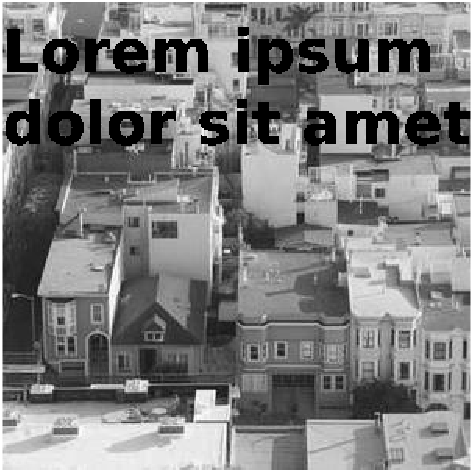
\includegraphics[width=0.32\linewidth]{\mapa/input.png}
    \caption{Slika z besedilom.}
\end{figure}

\begin{figure}[!ht]
    \begin{subfigure}{0.325\linewidth}
        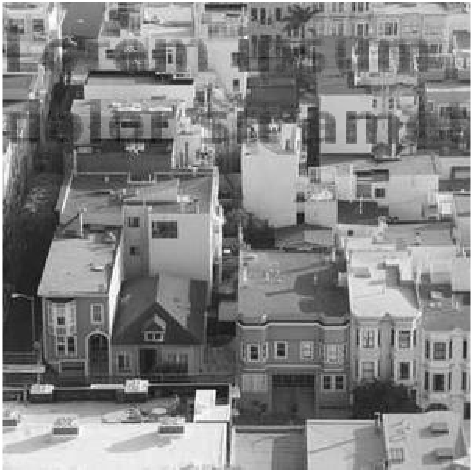
\includegraphics[width=\linewidth]{\mapa/rezSVT.png}
        \caption{Rekonstrukcija z algoritmom SVT.}
    \end{subfigure}
    \hfill
    \begin{subfigure}{0.325\linewidth}
        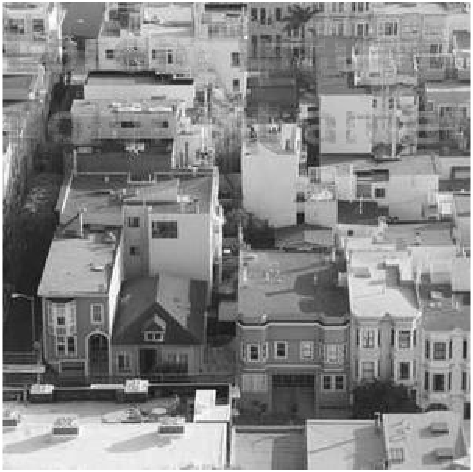
\includegraphics[width=\linewidth]{\mapa/rezTNNM.png}
        \caption{Rekonstrukcija z algoritmom TNNM.}
    \end{subfigure}
    \hfill
    \begin{subfigure}{0.325\linewidth}
        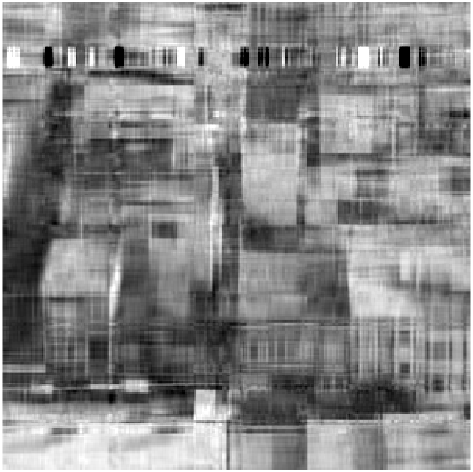
\includegraphics[width=\linewidth]{\mapa/rezLMaFit.png}
        \caption{Rekonstrukcija z algoritmom LMaFit.}
    \end{subfigure}
\end{figure}

\begin{table}[!ht]
    \centering
    \begin{tabular}{|c|c|c|}
    \hline
    & Napaka & Čas izvajanja (s) \\
    \hline
    SVT & $4.64 \times 10^{3}$ & 674s \\
    TNNM & $2.64 \times 10^{3}$ & 83.6s \\
    LMaFit & $3.17 \times 10^{3}$ & 0.95s \\
    \hline
    \end{tabular}
    \caption{Rezultati rekonstrukcije različnih algoritmov.}
\end{table}